
\chapter{Opdracht}

In dit hoofdstuk wordt beschreven bij welke organisatie de opdracht zich afspeelt. Wat waren de ontwikkelingen binnen de organisatie en wat zijn de redenen om een nieuw project te starten.

\section{Achtergrond}

Het bedrijf Shop2market is een software development bedrijf in de business-to-business sector. De organisatie helpt webwinkels online adverteren met als doelstelling de winstgevendheid van online advertenties te maximaliseren.
Voor alsnog diende shop2market als een IT oplossing ondersteunend aan het adviesbedrijf. Het merendeel van deze klanten zijn webwinkels in het A segment. Maar omdat de integratie met een webwinkel vaak maatwerk opleverde, duurde een integratie gemiddeld zes tot acht maanden. Hieruit valt ook te concluderen dat veel bedrijven niet de technologische middelen in huis hebben om zelfstandig te kunnen starten met adverteren.

Daarom werd in begin 2015 gestart met de ontwikkeling van Adcurve. Met de ervaring vanuit de adviesorganisatie zijn veel processen vertaald naar functionaliteiten om een self-service applicatie mogelijk te maken. De gewenste groei is nu mogelijk doordat webwinkels gebruik maken van hetzelfde webwinkel platform zoals SEOShop, Shopify of Magento.

Dit heeft als gevolg dat Shop2market nu webwinkels in het midden en klein bedrijf op internationaal bedienent maar met een groter volume. Webwinkels zijn nu binnen enkele minuten geïnstalleerd en kunnen hun producten gemakkelijk adverteren via zogeheten publishers. Deze kan de gebruiker zelf installeren binnen Adcurve wardoor het process geautomatiseerd word afgehaldend. Publishers zijn de bedrijven die de advertenties publiceren. De soort advertenties verschillen nogal per publisher. Denk bijvoorbeeld aan ingekochte zoekresultaten, producten op prijsvergelijkers of blogs (Affiliaties) of zelfs producten op marktplaatsen.

Zodra een gebruiker een publisher installeerd vindt er een volledige integratie plaats. Voor de webwinkel word de afkomstigheid van bezoekers en bestellingen gemeten. In combinatie met de advertentiekosten van publishers worden de nodige statistieken berekend. Met deze gegevens word de winstgevendheid van advertenties berekend. Door de div. functionaliteiten\footnote{Denk hierbij aan datavisualiasties en beheeracties, soms ook wel "Actionable insights" genoemd.} in Adcurve kan de webwinkel zijn online marketing campagnes controleren en binnen budget houden. Dit is mogelijk doordat Adcurve een partij is tussen de webwinkel en publishers.
\pagebreak

\section{Aanleiding} % de aanleiding tot de opdracht

Het afgelopen jaar zijn de meeste basis functionaliteiten voor Adcurve ontwikkeld. Daarnaast zijn er vijf publishers geintegreerd waar voor een volledige dataintegratie plaatsvindt. Bij deze publishers worden kosten niet door ons berekend o.b.v. een percentage of vast bedrag. De kosten die in rekening zijn gebracht worden gerapporteerd en door Adcurve geïmporteerd.
Omdat de belangrijkste functionaliteiten berusten op de beschikbaarheid van statistieken ligt dit proces aan de kern van het product. Helaas verloopt het importeren niet altijd zonder fouten. Het actief bewaken van datakwaliteit is hierdoor een prioriteit geworden. In de huidige situatie is dit nog lastig, doordat het berekenen van de statistieken een langdurig proces is.

De huidige strategie is om meer klanten aan te trekken door meer landen en industriën te ondersteunen. Het is te verwachten dat het aantal data integraties met publishers zal toenemen, en het probleem daardoor groter wordt. Daarnaast is de huidige situatie niet optimaal om mee te beginnen. De statistieken zijn s'middags pas beschikbaar, wardoor veel functionaliteiten werken met data van meer dan een dag oud. Er is hierdoor een een toenemende wens ontstaan om de huidige oplossing te herzien. Dit moet internationale groei van Adcurve onderstuenen, en ruimte bieden om functionaliteiten betrouwbaarder en te maken.

\section{Organisatie} % beschrijving van de organisatie van de opdrachtgever en de plaats van de student daarin

Shop2market is met een team tussen de 15 en 20 werknemers gevestigd in Hilversum. De organisatie kan naar de theorie van
\autocite{mintzberg} worden omschreven als een Adhocracy: “Door de innovatieve aard van projecten is een organisatie gebaat bij flexibiliteit. Een formele hiërarchische structuur werkt daardoor minder goed.” Dit is herkenbaar en valt terug te leiden naar de professionele houding die van werknemers word verwacht. Er word autonomie gegeven om zelf structuur aan te brengen wanneer dit nodig is.

\begin{figure}[h]
    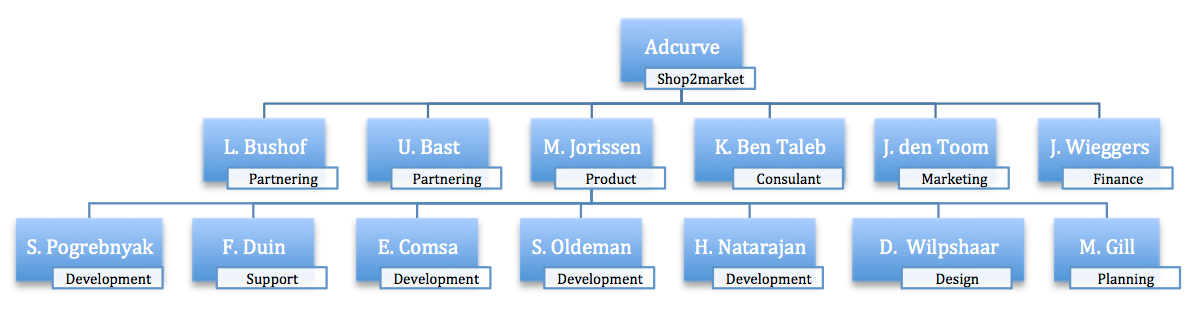
\includegraphics[width=1\textwidth]{organisation_structure.png}
    \caption{Organogram waarin het team en de relaties binnen Shop2market worden afgebeeld.}
    \label{fig:orgchart}
\end{figure}

\pagebreak

\section{De kwestie} % een kwestie (aanleiding, het op te lossen probleem, de te vervullen behoefte of de te benutten kans);

Zoals te lezen valt in de de aanleiding zijn meerdere redenen voor dit project.

\begin{enumerate}
    \item De tijd die het kost om statistieken te berekenen is aan de hoge kant. De berekeningen worden uitgevoerd met behulp van MongoDb MapReduce. Het team voorziet dat deze technologie niet genoeg schaalbaarheid bied. Dit omdat rekentijd linear is toegenomen in relatie tot de hoeveelheid data. Met de verwachte groei van Adcurve komen nieuwe requirements aan het licht en er moet naar een nieuwe oplossing worden gezocht.
    \item Bij voorkeur worden publishers geintegreerd met behulp van API's oftewijl; een externe databron. Op deze manier worden berekeningen uitgevoerd met preciese advertentiekosten. Maar doordat externe factoren nu een rol spelen in de berekeningen is het niet te garanderen dat de de uitkomst altijd correct is. Zodra fouten intern of extern hersteld zijn worden berekeningen voor een bepaalde dag, webwinkel of publisher opnieuw uitgevoerd. Het uitvoeren van dit soort correcties zijn tijdrovend door de huidge implementatie en gebruikte technieken.
    \item Als laatste onstaat er een kans door de huidige problematiek op te lossen. Webwinkels ontvangen tot soms tot 30 dagen na een bestelling een retournering van een of meerdere producten. Dit betekend dat een product niet verkocht is en de omzet uit de bestelling lager ligt dan is berekend. Het is wenselijk om berekende statestieken met betrekken tot retour bestellingen opnieuw te berekenen.
\end{enumerate}


\section{Doelstellingen} % de doelstellingen (wat moet na afloop van het afstudeerproject zijn bereikt);

In het kort moeten webwinkeleigenaren in staat zijn om beslissingen te maken op basis van correcte en actuele gegevens in Adcurve. Dit betekend dat de gegevens die Adcurve toont altijd te verklaren zijn en overeenkomen met de werkelijkheid. Als voorbeeld hiervan zijn gegevens over de vorige dag voor kantooruren beschikbaar en worden retouropdrachten ook verwerkt in Adcurve. Als laatste moeten gegevens accuraat en betrouwbaar zijn, tenzij anders vermeld staat. Daarom moet tijdig herstel van fouten mogelijk zijn.

\section{Type opdracht}

Aan de hand van beschikbare technieken wordt er gekozen een aantal mogelijk oplossingen\newline te proberen middels een Proof of Concept. Dit sluit goed aan bij de aard van een onderzoeksopdracht. Door dit onderzoek moet duidelijk gaan worden: hoe de oprdacht kan worden opgelost, of dit mogelijk is en wat er nodig is om de oplossing naar productie te brengen. Door de opdrachtgever is gevraagd om een aantal POC's te ontwikkelen om tot een inzicht over de oplossing te komen. Er is hierdoor sprake van een ontwikkel opdracht.

